\section{\ieeemac{}}
\ieeemac{} is a standard that defines the physical layer
(PHY) and media access control (MAC) for Low Rate
Wireless Personal Area Networks (LR-WPANs),
targeting devices constrained by low computing
power, memory and energy \cite{salmanOverviewIEEE8021542010}. It is
designed to operate in Personal
Operating Space (POS) of 10 meters or less and supports
three types of topology: star, peer-to-peer and mesh (a network that
connects a large number of nodes through relaying messages). The
standard offers three free bands
throughout the world with the throughput of 250\,kbps in the 2.4\,GHz
band 40\,kbps at 915\,MHz and 20\,kbps at 868\,MHz.

The 802.15.4 standard controls channel access with Carrier-Sense
Multiple Access with
Collision Avoidance (CSMA/CA). It defines two mode:
beacon-enabled for synchronous access and non-beacon-enabled for
asynchronous access.

In non-beaconed-enabled mode, nodes use unslotted
CSMA/CA, and they do not exchange request-to-send (RTS) and clear-to-send (CTS)
messages. When a node has packets to send, it delays the transmission for a
random backoff period. Afterward, it senses the medium and transmit
only if the channel is idle. If the channel is busy, the node waits for
another random backoff period and check the channel again.
Because transmissions are not synchronised, packets can arrive at any
time. As a result, nodes that may receive data have to keep their
radio on at all time.
This is especially costly in multihop topologies where nodes must
relay messages for other nodes.

In beacon-enabled mode, the coordinator cuts time into superframes,
which consists of 16 equally sized slots. Each
superframe starts when the coordinator sends a beacon to synchronise
the nodes. Each superframe has an active period and an optional
inactive period. During the active period, nodes compete for the
channel using slotted CSMA/CA, with backoff period aligned to the
slot boundary. During the inactive period, nodes can turn off their
radios until the next beacon to save energy.

\section{\ieeemacE{} Time-Slotted Channel Hopping}
The IEEE 802.15.4e amendment introduced Time-Slotted Channel Hopping
(TSCH), a MAC behavior that provides high reliability and time
critical assurances \cite{tsch}. TSCH achieves this by
combining time-division multiple access (TDMA) with frequency hopping.
Time is divided into fixed-length timeslots, and a group of
consecutive timeslots forms a \emph{slotframe}, which repeats
periodically. Nodes also switch channels from one timeslot to the
next according to a hopping sequence, as illustrated in
Figure~\ref{fig:tsch}. Spreading transmissions across channels in
this way reduces the effect of interference and multipath fading on
any single channel.

\begin{figure}
    \begin{center}
        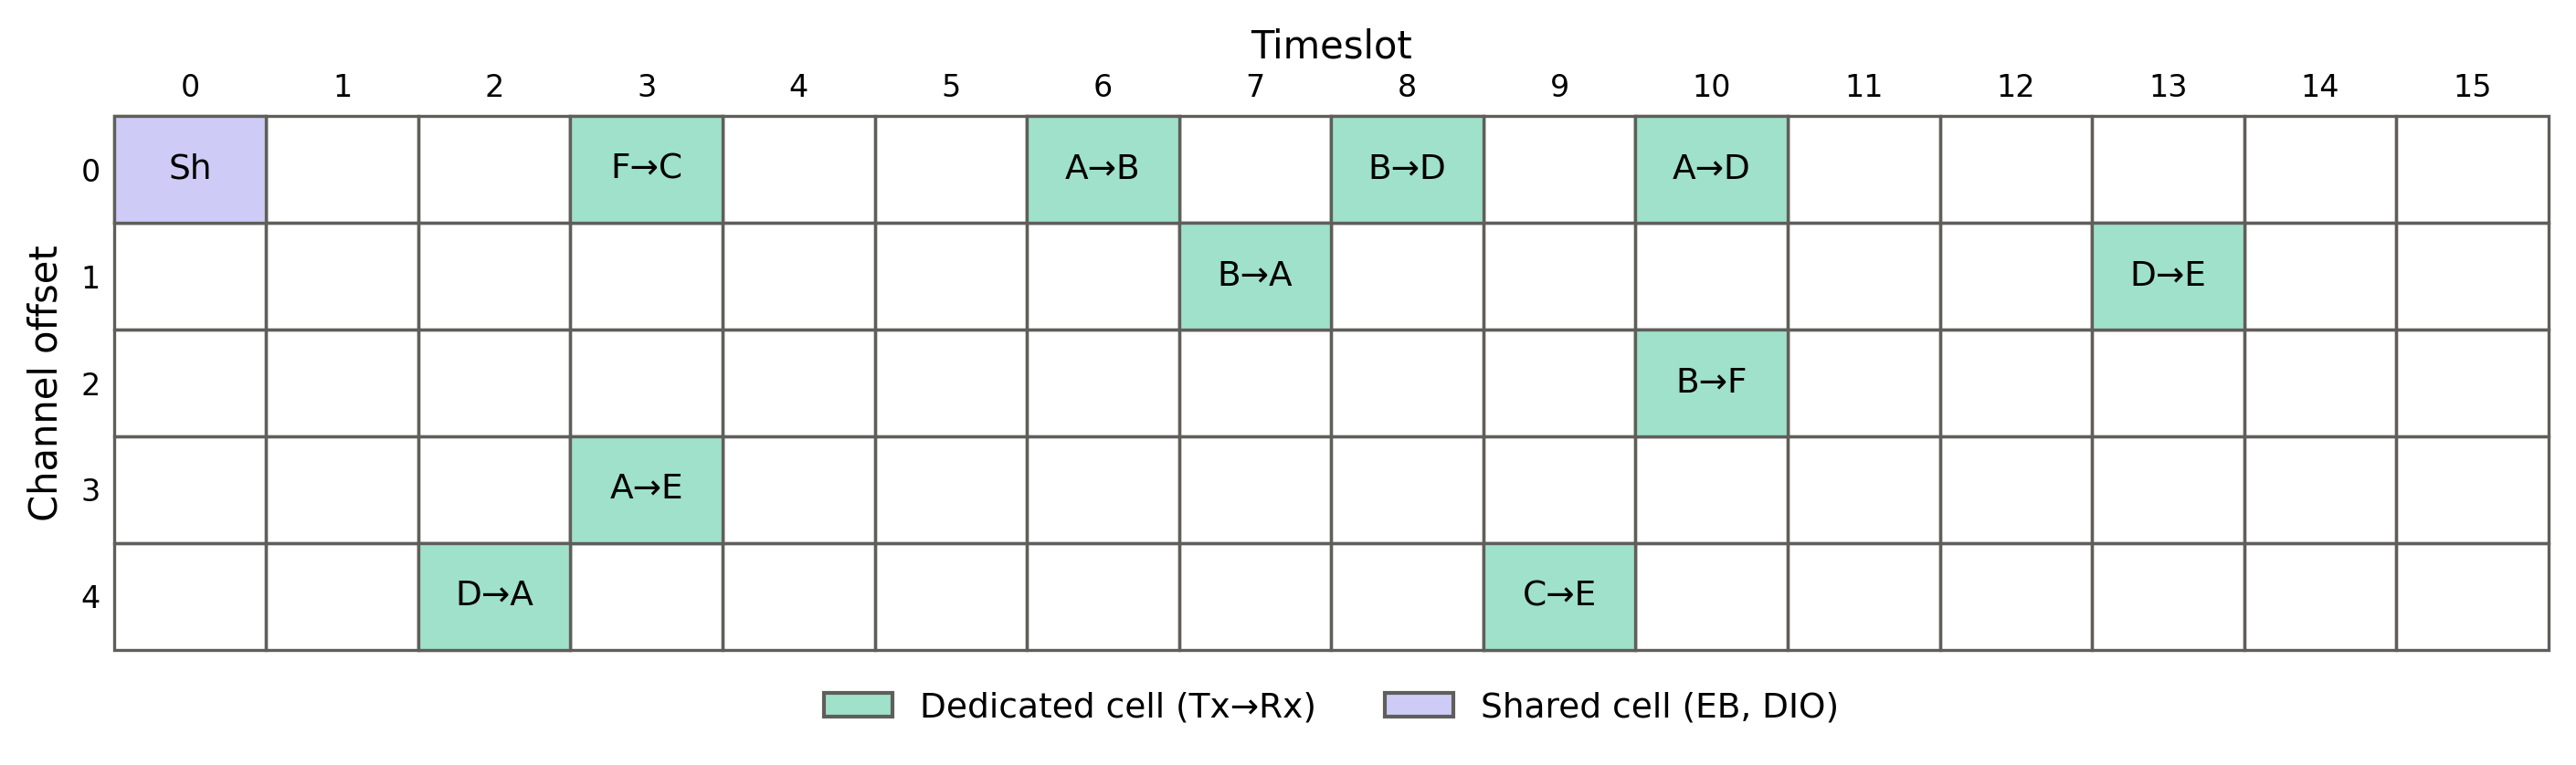
\includegraphics[width=0.9\textwidth]{assets/TSCH.png}
    \end{center}
    \caption{TSCH time slot visualisation.}\label{fig:tsch}
\end{figure}

A timeslot must be long enough that transmission and acknowledging
can be done within the duration of a slot. In each
timeslot, a node either transmits, receives or sleeps. A node with a
frame to send waits for a timeslot in which it is scheduled to
transmit, and then starts sending at a fixed offset from the start of
the slot. A node scheduled to receive turns on its radio shortly
before the expected start of the frame. If the node senses that it
does not have any data to receive after a short guard time, it turns its
radio off again for the rest of
the slot to save energy.

TSCH also uses channel hopping, so successive transmissions over the
same link use different frequencies. Each link is assigned a
channel offset, which lets different nodes communicate at the same time on
different channels. The frequency $f$ used for a transmission in that
link is
\begin{equation}
    f = F\left[(\mathit{ASN} + \mathit{channel\ Offset}) \bmod
    n_{\mathit{channel}}\right],
\end{equation}
where $n_{\mathit{channle}}$ is the number of available channels (16 in
the 2.4\,GHz band), Absolute Slot Number (ASN) is the total number of
timeslots that have elapsed since the network started
and $F$ is a lookup table that maps an index to a
physical channel.

TSCH avoids collisions through its schedule. Each transmission
occupies a \emph{cell}, identified by a slot offset within the
slotframe and a channel offset. In a \emph{dedicated} cell, only one
transmitter is scheduled, so the transmission is free of collision.
In a \emph{shared} cell, several nodes may transmit, and collisions
are handled by a CSMA/CA-like backoff. However, \ieeemacE{} does
not specify how the schedule is built or maintained, and leaves this
task to higher layers. One example is the approach of the IETF 6TiSCH
working group, which defines the 6TiSCH Operation Sublayer (6top)
\cite{rfc8480}, which lets neighboring nodes add and remove cells,
and the Minimal Scheduling Function (MSF) \cite{rfc9033}, which
decides when to do so.

Compared with CSMA/CA, TSCH offers higher reliability and lower
energy consumption. Reliability comes from two mechanisms: channel
hopping to reduce the impact of interference and multipath fading on
any single channel, and dedicated cells to allow nodes to transmit
simultaneously while avoiding collisions. The lower
energy consumption comes from nodes turning on their radio only in the
timeslots in which they are scheduled, and keep the radio off for the rest
of the slotframe.

These benefits come at a cost. TSCH is more complex than CSMA/CA: it
requires network-wide time synchronisation, which nodes must maintain
by periodically exchanging packets with their time source, and it
requires a schedule to be built and maintained. TSCH also introduces
latency, because a node with a packet to send must wait for its next
scheduled cell. The length of the slotframe therefore sets a
trade-off: a short slotframe gives nodes more frequent transmission
opportunities and lower delay, but forces them to wake up more often
and consume more energy

\section{IPv6 over Low-Power Wireless Personal Area Networks (6LoWPAN)}
Before 6LoWPAN, low-power wireless networks relied on proprietary or
non-IP protocol stacks such as ZigBee, since IP was considered too
demanding in computation and memory for constrained devices
\cite{culler20096lowpan}. Connecting these networks to the Internet
required gateways that translated between their protocols and IP,
which added complexity and limited interoperability.

% TODO: direct sentence, 6LoWPAn introduce bridge between layers...
6LoWPAN (IPv6 over Low-Power Wireless Personal Area Networks) brings
IPv6 to these devices, specifically to networks built on the
\ieeemac{} PHY and MAC layers \cite{rfc4944}. Using IPv6 end to end
simplifies interconnection with other networks and removes the need
for protocol-translating gateways. It also allows existing,
well-developed IP tools to be used for commissioning, configuring,
managing and debugging these networks.

Running IPv6 directly over \ieeemac{} is impractical because the two
were designed under very different assumptions. IPv6 targets
high-bandwidth links with large frames, requiring a minimum Maximum
Transmission Unit (MTU) of
1280 bytes, whereas \ieeemac{} targets low-power devices, with frames
of at most 127 bytes and data rates of up to 250\,kbps. To bridge
this gap, 6LoWPAN introduces an adaptation layer between the IPv6
network layer and the \ieeemac{} MAC layer, which provides three main
functions:

\begin{itemize}
    \item \textbf{Header compression.} An uncompressed IPv6 header
        occupies 40 bytes, which is a large share of a 127-byte
        \ieeemac{} frame.
        Many of its fields are either constant or can be derived from
        other layers; for example, the source and destination addresses
        can often be reconstructed from the link-layer addresses. 6LoWPAN
        omits or shortens these fields to reduce header size.
    \item \textbf{Fragmentation and reassembly.} IPv6 requires every
        link to support a minimum MTU of 1280 bytes, whereas an
        \ieeemac{} frame carries at most 127 bytes. 6LoWPAN splits
        IPv6 datagrams that do not fit into a single frame into
        fragments and reassembles them at the receiver.
    \item \textbf{Link-layer forwarding.} 6LoWPAN optionally supports
        forwarding packets across multiple hops at the link layer
        (\emph{mesh-under}). Alternatively, routing can be performed at
        the IP layer (\emph{route-over}), which is the approach taken by
        RPL.
\end{itemize}
